\documentclass{beamer}

\usepackage{amsmath, amssymb}
\usepackage{graphicx}
\usepackage{url}
\usepackage{xspace}
\usepackage{pifont}
\usepackage{minted}
\usepackage{verbatim}
\usepackage{wasysym}
\usepackage[notocbib]{apacite}
\usepackage{bm}

\usetheme{AnnArbor}
\usefonttheme[onlymath]{serif}


\DeclareMathOperator{\Tr}{Tr}
\DeclareMathOperator*{\argmin}{arg\,min}

\title[PnS2018]{\textbf{PnS 2018} \\
\textbf{\normalsize Deep Learing with Raspberry Pi}\\
\normalsize Session 2}
\author{PnS 2018 Team}
\institute[INI-UZH/ETHz]{Institute of Neuroinformatics \\
University of Z\"urich and ETH Z\"urich}

\date{}

\begin{document}

\titlepage

\begin{frame}
\frametitle{Outline}

\tableofcontents
\end{frame}

% \AtBeginSection[]
%   {
%      \begin{frame}
%      \frametitle{Outline}
%      \tableofcontents[currentsection]
%      \end{frame}
%   }

% \section{Introduction}

% \begin{frame}[fragile]
%   \frametitle{Suggest Readings}
%
%   \begin{itemize}
%     \item[\ding{45}] CS229 lecture notes 1 and 4:
% \begin{verbatim}
% http://cs229.stanford.edu/notes/cs229-notes1.pdf
% http://cs229.stanford.edu/notes/cs229-notes4.pdf
% \end{verbatim}
%     \item[\ding{45}] Pattern Recognition and Machine Learning: Chapter 1 and 2.
%     \item[\ding{45}] Machine Learning: A probabilistic perspective: Chapter 1 and 2.
%     \item[\ding{45}] CS231n: Image Classification: Data-driven Approach, k-Nearest Neighbor, train/val/test splits
%
%       \url{http://cs231n.github.io/classification/}
%   \end{itemize}
% \end{frame}
%
% \begin{frame}
%   \frametitle{Suggested Readings Continued}
%
%   \begin{itemize}
%     \item[\ding{45}] UFLDL Tutorial: \href{http://ufldl.stanford.edu/tutorial/supervised/LogisticRegression/}{Logistic Regression}, \href{http://ufldl.stanford.edu/tutorial/supervised/SoftmaxRegression/}{Softmax Regression} and \href{http://ufldl.stanford.edu/tutorial/supervised/OptimizationStochasticGradientDescent/}{Stochastic Gradient Descent}.
%     \item[\ding{45}] CS231n: \href{http://cs231n.github.io/linear-classify/}{Linear classification: Support Vector Machine, Softmax} and \href{http://cs231n.github.io/optimization-1/}{Optimization: Stochastic Gradient Descent}.
%     \item[\ding{45}] \href{http://www.iro.umontreal.ca/~bengioy/dlbook/numerical.html}{DL Book Chapter 4 Numerical Computation 4.3} \href{http://www.iro.umontreal.ca/~bengioy/dlbook/optimization.html}{DL Book Chapter 8 Numerical Optimization 8.3}
%   \end{itemize}
% \end{frame}

\section{Learning Algorithms}

\begin{frame}
  \frametitle{Definition of a Learning Algorithm}

  ``A computer program is said to learn from
  \begin{itemize}
    \item[\checkmark] experience $E$ with respect to
    \item[\checkmark] some class of tasks $T$ and
    \item[\checkmark] performance measure $P$,
  \end{itemize}
  if its performance at tasks in $T$, as measured by $P$, improves with experience $E$'' \cite{mitchelltm1997}

\end{frame}

\begin{frame}
  \frametitle{The task $T$}

  \begin{description}
    \item[Classification] specify which $k$ categories some input belongs to. ($f: \mathbb{R}^{n}\rightarrow \{1,\ldots,k\}$)
    \item[Regression] predict a numerical value given some input. ($f: \mathbb{R}^{n}\rightarrow\mathbb{R}$)
    \item[Transcription] output a sequence of symbols, rather than a category code. (similar to classification, \emph{e.g.} speech recognition, machine translation, image captioning)
    \item[Denoising] predict \emph{clean} samples $\bm{x}$ from \emph{corrupted} samples $\tilde{\mathbf{x}}$ (estimate $P(\mathbf{x}|\tilde{\mathbf{x}})$).
  \end{description}

\small
\emph{Many more types are not listed here.}
\end{frame}

\begin{frame}
  \frametitle{The performance measure $P$}

  \begin{itemize}
    \item[\ding{226}] Measure $P$ is usually specific to the task $T$. (\emph{e.g.} accuracy to classification)
    \item[\ding{226}] Batches of unseen \emph{test} data is introduced to measure performance.
    \item[\ding{226}] Design measure $P$ can be very subtle. It should be effective.
  \end{itemize}
\end{frame}

\begin{frame}
  \frametitle{The experience $E$}

  \emph{Experience is what learning algorithms are allowed to have during learning process.}

  \begin{itemize}
    \item[\ding{229}] Experience is usually an \emph{dataset}, a collection of \emph{examples}.
    \item[\ding{229}] \emph{Unsupervised learning algorithms} experience a dataset containing many features, learning useful structure of the dataset (estimate $p(\mathbf{x})$).
    \item[\ding{229}] \emph{Supervised learning algorithms} experience a dataset containing features, but each example is also associated with a \emph{label} or \emph{target} (estimate $p(\mathbf{y}|\mathbf{x})$).
  \end{itemize}
  
\end{frame}

\section{Linear Regression}

\begin{frame}
  \frametitle{Problem Description}

  The \emph{task} is to build a system that can take a vector $\mathbf{x}\in\mathbb{R}^{n}$ as input and predict the value of a scalar $y\in\mathbb{R}$ as its output. Let $\hat{y}$ be the value that out model predicts $y$ should take on. We define the output to be
  \begin{equation*}
    \hat{y}=\mathbf{w}^{\top}\mathbf{x}+b
  \end{equation*}
  where $\mathbf{w}\in\mathbb{R}^{n}$ is a vector of parameters and $b$ is a bias term.
\end{frame}

\begin{frame}
  \frametitle{Performance Measure and Experience}

  The \emph{experience} contains a set of training examples where each sample is a pair of input and output $(\mathbf{x}, y)$.

  One \emph{performance measure} here can apply is \emph{mean squared error} of the model on test set. Let test example as $\mathbf{x}^{(\text{test})}$ and regression targets as $\mathbf{y}^{(\text{test})}$, $\hat{\mathbf{y}}^{(\text{test})}$ is the predictions of the model on the test set, the mean square error is given by:
  \begin{equation*}
      \text{MSE}_{\text{test}}=\frac{1}{N}\sum_{i=1}^{N}(\hat{\mathbf{y}}^{(\text{test})}-\mathbf{y}^{(\text{test})})_{i}^{2}.
  \end{equation*}
\end{frame}

\section{Logistic Regression}

\begin{frame}
  \frametitle{Logistic Function}

  \begin{align*}
    \sigma(\mathbf{x})&=\frac{1}{1+\exp(-\mathbf{W}^{\top}\mathbf{x}+b)} \\
    p(y=1|\mathbf{x})&=\sigma(\mathbf{x})\\
    p(y=0|\mathbf{x})&=1-\sigma(\mathbf{x})
  \end{align*}
\end{frame}

\begin{frame}
  \frametitle{Logistic Regression --- Binary Classifier}

  \begin{align*}
    J(\theta)&=-\frac{1}{N}\sum_{i}\left(y^{i}\log(P(y=1|\mathbf{x}^{i}))+(1-y^{i})\log(p(y=0|\mathbf{x}^{i}))\right) \\
    \theta^{\star}&=\argmin_{\theta}J(\theta)
  \end{align*}
\end{frame}

% \section{Softmax Regression}
%
% \begin{frame}
%   \frametitle{Extending Logistic Function --- Softmax Function}
%
%   \begin{equation*}
%       P(y=k|\mathbf{x}; \mathbf{W})=\frac{\exp(\mathbf{W}^{(k)\top}\mathbf{x}+b_{k})}{\sum_{j=1}^{K}\exp(\mathbf{W}^{(j)\top}\mathbf{x}+b_{k})}
%   \end{equation*}
% \end{frame}
%
% \begin{frame}
%   \frametitle{Softmax Regression --- Multi-classes Classifier}
%
%   \begin{align*}
%       J(\theta)&=-\frac{1}{N}\sum_{i=1}^{N}\sum_{k=1}^{K}\mathbf{1}\{y^{i}=k\}\log P(y^{i}=k|\mathbf{x}^{i}, \theta) \\
%       \theta^{\star}&=\argmin_{\theta}J(\theta)
%   \end{align*}
% \end{frame}

\section{Generalization, Capacity, Overfitting and Underfitting}

% \begin{frame}
%   \frametitle{Generalization, Capacity, Overfitting, Underfitting}
%
%   \begin{description}
%     \item[Generalization] ability to perform well on previously unobserved inputs.
%     \item[Capacity] ability to fit a wide variety of functions.
%     \item[Overfitting] occurs when the gap between training error and test error is too large
%     \item[Underfitting] occurs when the model is not able to obtain a sufficiently low error value on the training set.
%   \end{description}
% \end{frame}

\begin{frame}
  \frametitle{Generalization, Capacity, Overfitting, Underfitting}

  \begin{figure}
    \centering
    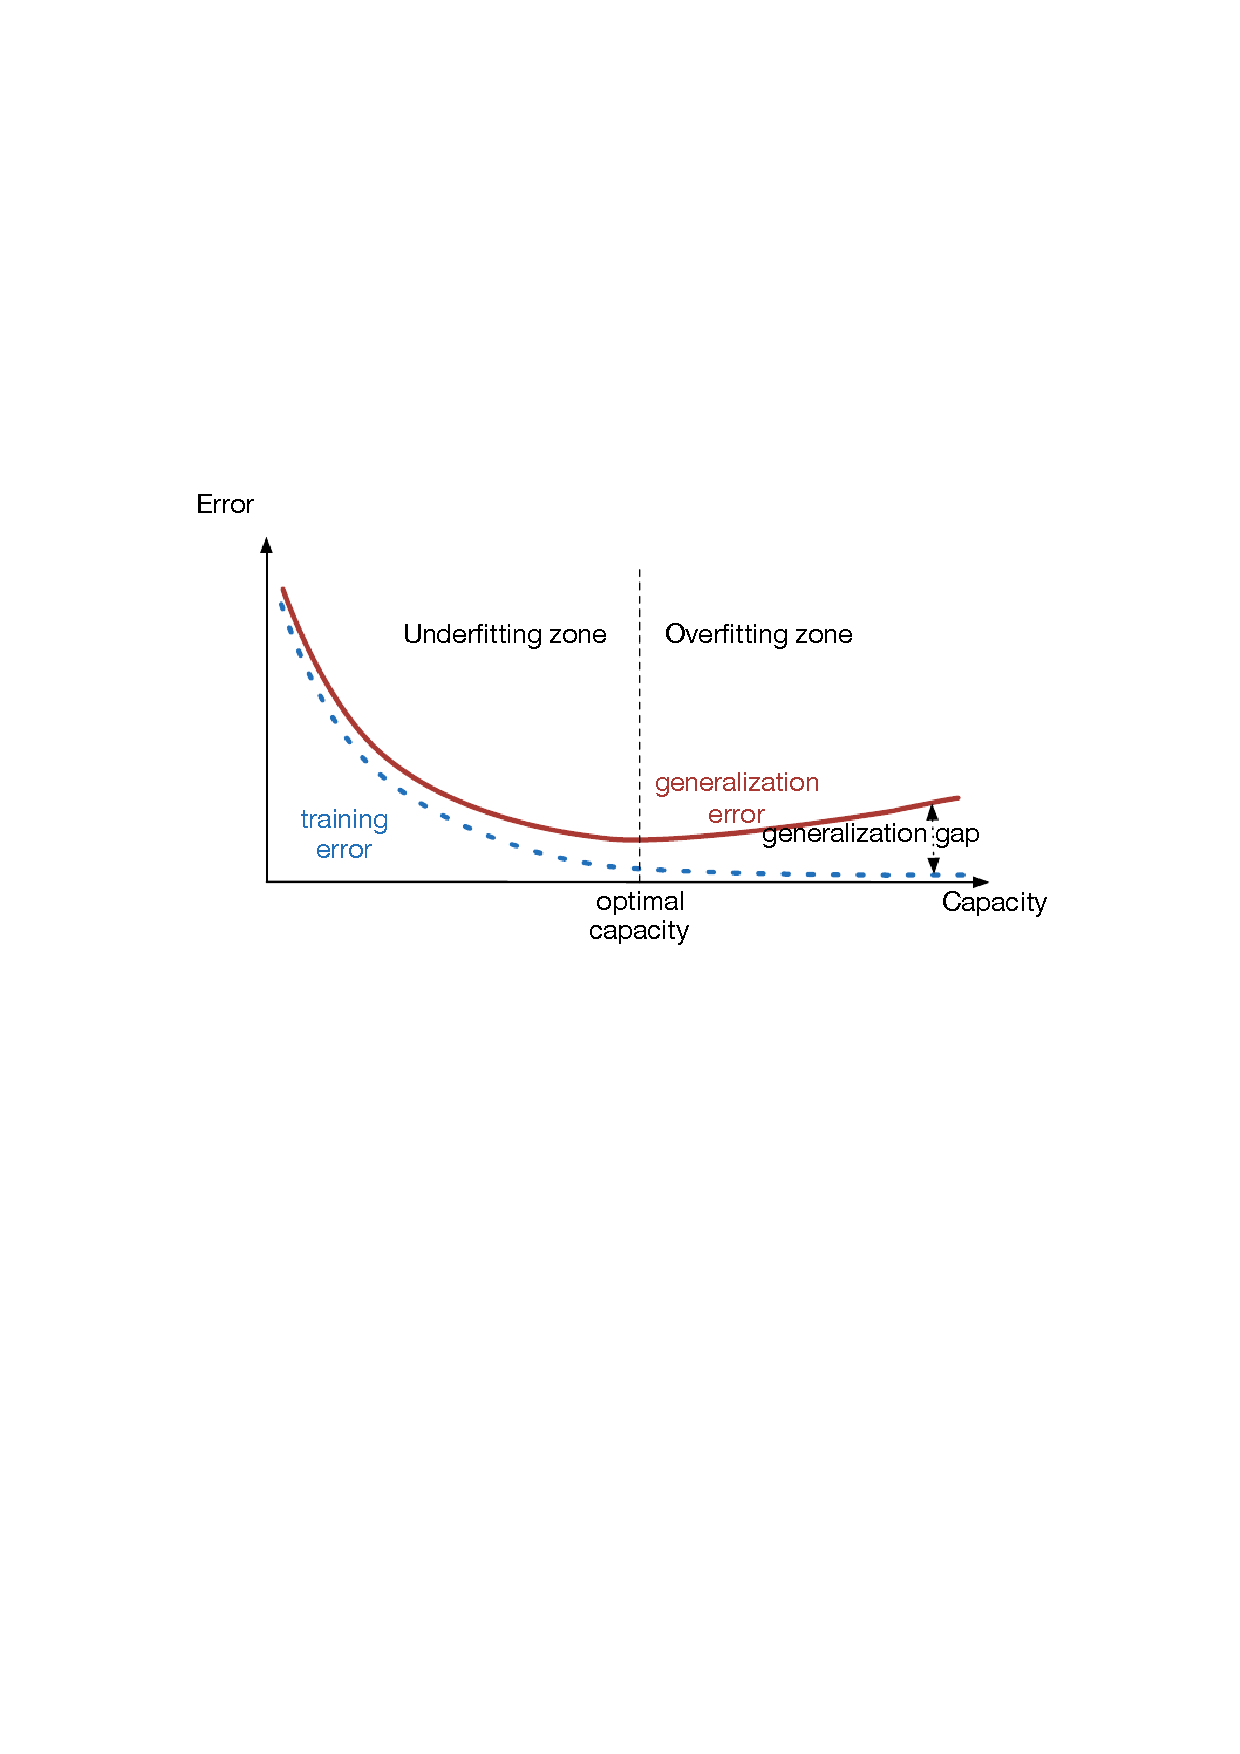
\includegraphics[width=0.8\textwidth]{relationships_between_terms.pdf}
  \end{figure}
\end{frame}

\begin{frame}
  \frametitle{No Free Lunch Theorem}

  \begin{quote}
    The no free lunch theorem for machine learning \cite{Wolpert:1996} states that, averaged over all possible data generating distributions, every classification algorithm has the same error rate when classifying previous unobserved points. In some sense, no ML algorithm is universally any better than any other.
  \end{quote}

  \centering
  \textbf{Seek solution for some relevant distributions, NOT universal distribution.}
\end{frame}

% \begin{frame}
%   \frametitle{Hyperparameters, Validation Sets}
%
%   \begin{description}
%     \item[Hyperparameters] settings that control the behavior of the learning algorithm. Usually choose empirically.
%       \item[Validation Sets] Subset of data used to guide the selection of hyperparameters. (split from training dataset, usually 20\%)
%   \end{description}
% \end{frame}

% \begin{frame}
%   \frametitle{Curse of Dimensionality}
%
%   Many machine learning problem become exceedingly difficult when the number of dimensions in the data is high. The phenomenon is known as the \emph{curse of dimensionality}. Of particular concern is that the number of possible distinct configurations of the variables of interest increases \textbf{exponentially} as the dimensionality increases.
% \end{frame}

\begin{frame}
  \frametitle{Curse of Dimensionality}

  \begin{figure}
    \centering
    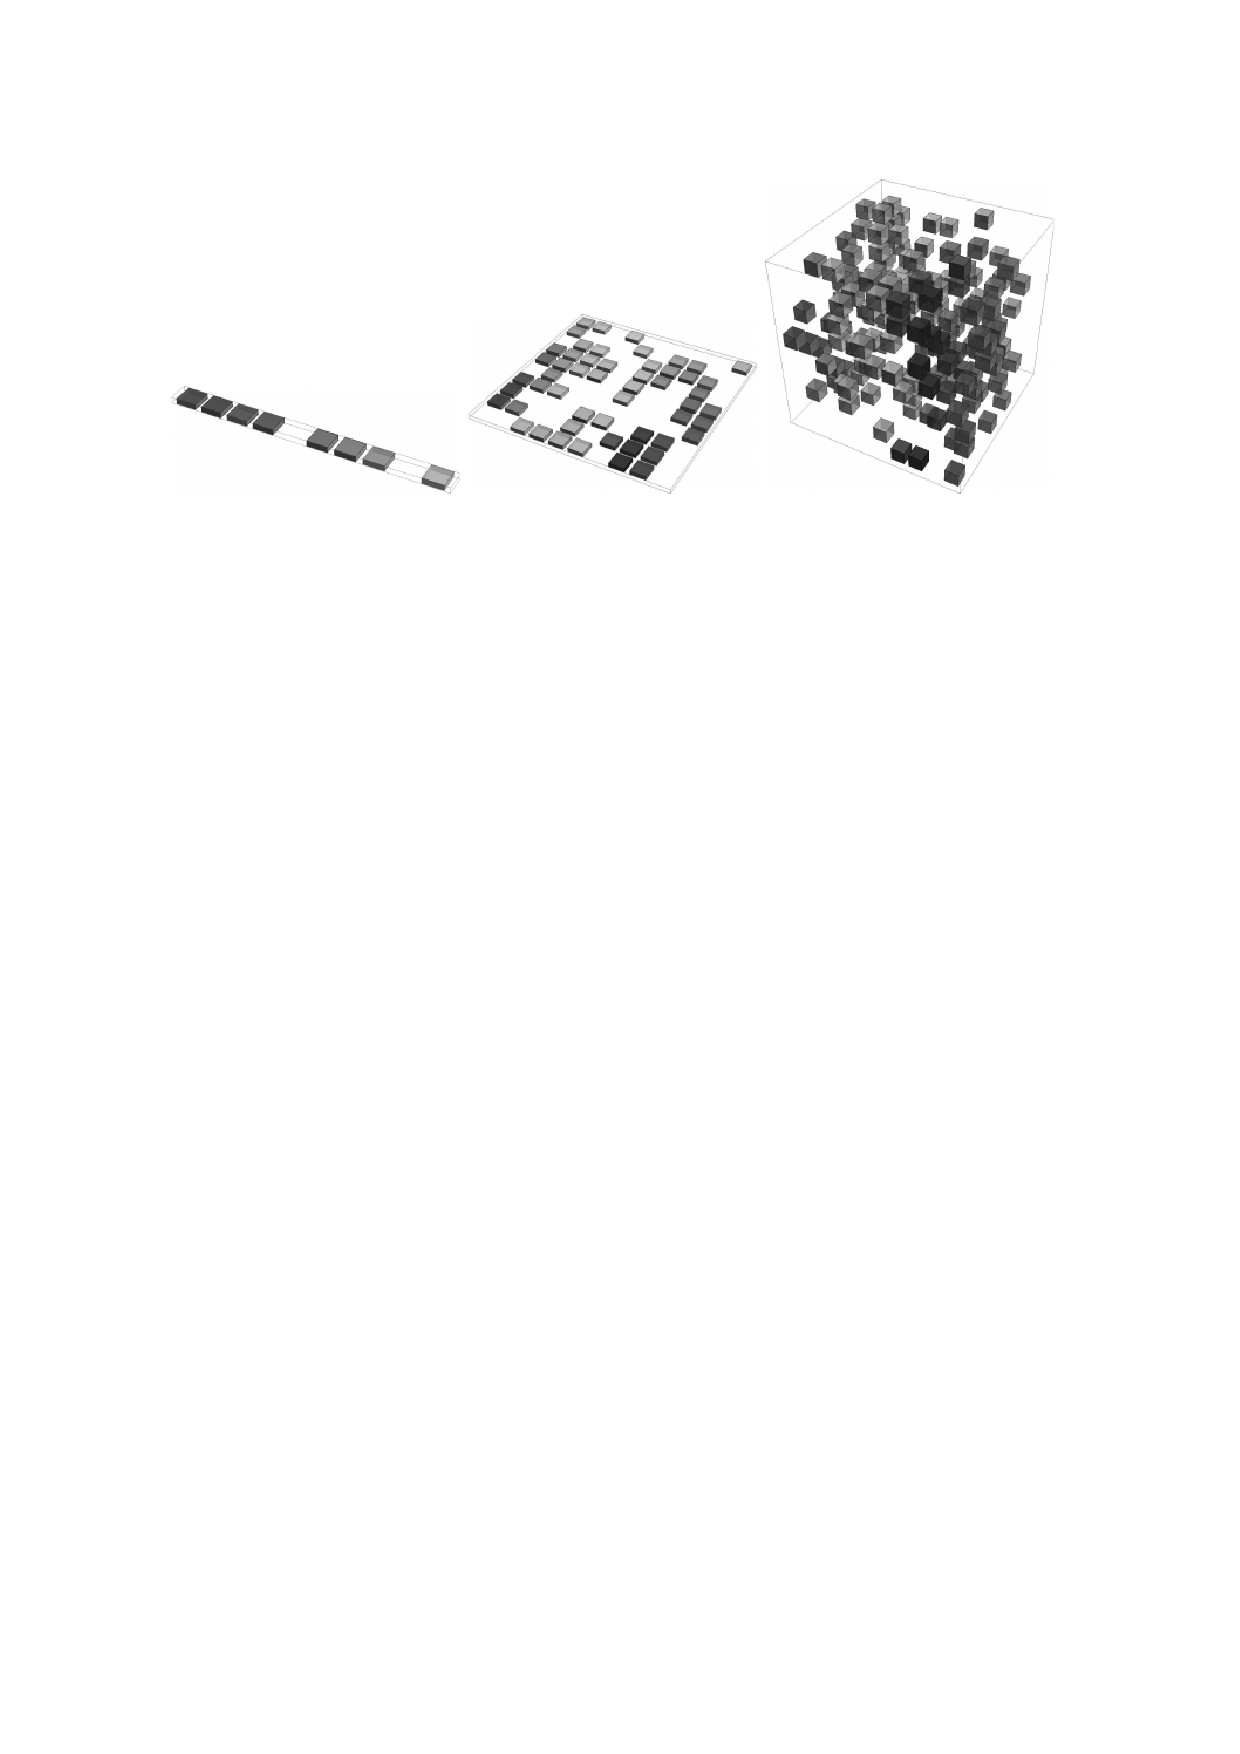
\includegraphics[width=0.8\textwidth]{curse_of_dimensionality.pdf}
  \end{figure}
\end{frame}

\section*{Q\&A}
\begin{frame}
  \frametitle{Q\& A}
  \begin{figure}
    \centering
    
\includegraphics[width=0.5\textwidth]{machine_learning_logo.png}
  \end{figure}
\end{frame}



\section{Stochastic Gradient Descent}

\begin{frame}
  \frametitle{Cost}
  \begin{itemize}
    \item Target: to learn some optimal parameters $\theta$
    \item Strategy: to minimize some cost $L$ respect to $\theta$
    \item Cost choice: cross-entropy cost, mean-squared error cost
    \item Solution: Gradient Descent!
  \end{itemize}
\end{frame}

\begin{frame}
  \frametitle{Gradient optimization}
  \begin{figure}
    \centering
    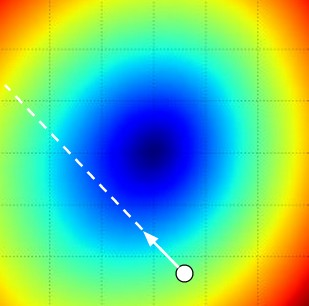
\includegraphics[width=0.5\textwidth]{stepsize.jpg}
  \end{figure}

  \href{http://rt.dgyblog.com/res/dlworkshop/opt1.gif}{Demo 1}; \href{http://rt.dgyblog.com/res/dlworkshop/opt2.gif}{Demo 2}
\end{frame}

\begin{frame}
  \frametitle{Stochastic Gradient Descent (SGD)}

  \begin{equation*}
    \theta^{*}=\theta-\alpha\frac{\partial}{\partial \theta}J(\theta)
  \end{equation*}
\end{frame}


\begin{frame}
  \frametitle{Variants: momentum SGD}

  \begin{align*}
    V^{*}&=\mu V+\alpha\nabla L(\theta) \\
    \theta^{*}&=\theta-V^{*}
  \end{align*}
\end{frame}

% \begin{frame}
%   \frametitle{Variants: Nesterov's Accelerated Gradient (NAG)}
%   \begin{align*}
%     V^{*}&=\mu V-\alpha\nabla L(\theta+\mu V) \\
%     \theta^{*}&=\theta+V^{*}
%   \end{align*}
% \end{frame}

\section*{Q\&A}

\begin{frame}
  \frametitle{Q\&A}
  \begin{figure}
    \centering
    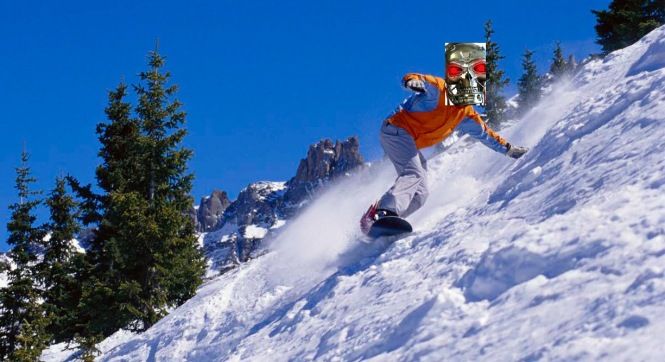
\includegraphics[width=0.7\textwidth]{gradient_descent.jpg}
  \end{figure}
\end{frame}


\begin{frame}[allowframebreaks]
\frametitle{References}
\footnotesize
\bibliographystyle{apacite}
\bibliography{../dlworkshopref}
\end{frame}

\end{document}
%%% Local Variables:
%%% mode: latex
%%% TeX-master: t
%%% End:
